\begin{figure}
    \begin{subfigure}{.45\textwidth}
          \centering
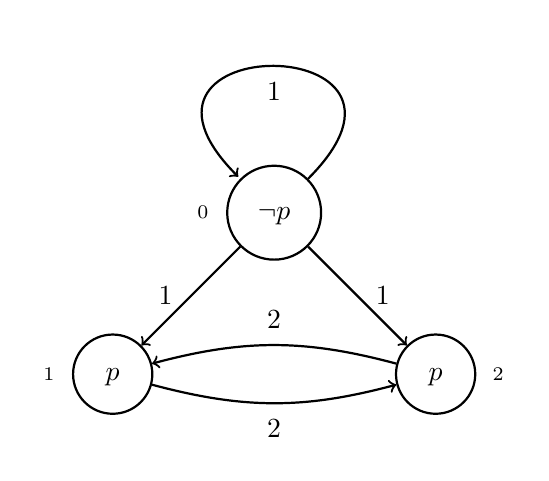
\begin{tikzpicture}[->,circle,draw,node distance=2.9cm
                   ]

    \node[circle,label=180:$\st_0$,draw,thick](w0){$
        \begin{array}{c}       
            \neg p\\
        \end{array}
    $};
    \node[circle,label=0:$\st_2$,below right of=w0,draw,thick](w1) {$
        \begin{array}{c}       
            p\\
        \end{array}
    $};
    \node[circle,label=180:$\st_1$,below left of=w0,draw,thick](w2) {$
        \begin{array}{c}       
            p\\
        \end{array}
    $};
    \path[thick] (w0) edge [right] node {1} (w1)
    (w0) edge [below,loop] node {1} (w0)
    (w1) edge [above,bend right=15] node {2} (w2)
    (w2) edge [below,bend left=345] node {2} (w1)
    (w0) edge [left] node {1} (w2);

\end{tikzpicture} 
              \caption{Kripke model}
                \label{example_nottree}
    \end{subfigure}%
    \begin{subfigure}{.5\textwidth}
          \centering
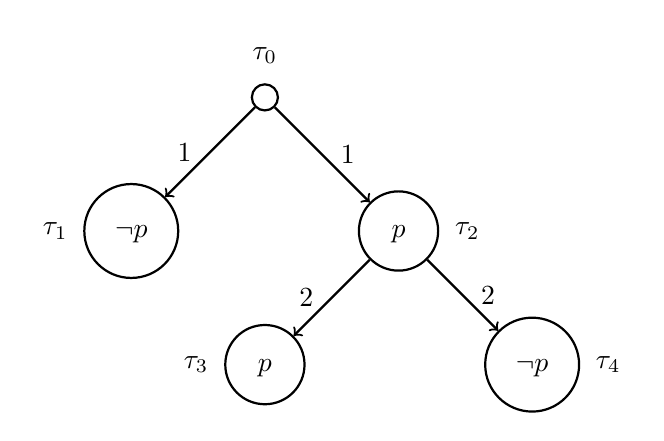
\begin{tikzpicture}[->,circle,draw,node distance=2.4cm,fill=black
                   ]

    \node[circle,label=90:$\tau_0$,draw,thick](w0){$
    $};
    \node[circle,label=180:$\tau_1$,below left of=w0,draw,thick](w1) {$
        \begin{array}{c}       
            \neg p\\
        \end{array}
    $};
    \node[circle,label=0:$\tau_2$,below right of=w0,draw,thick](w2) {$
        \begin{array}{c}       
            p\\
        \end{array}
    $};
    \node[circle,label=180:$\tau_3$,below left of=w2,draw,thick](w3) {$
        \begin{array}{c}       
            p\\
        \end{array}
    $};
    \node[circle,label=0:$\tau_4$,below right of=w2,draw,thick](w4) {$
        \begin{array}{c}       
            \neg p\\
        \end{array}
    $};
    \path[thick] (w0) edge [left] node {1} (w1)
    (w0) edge [right] node {1} (w2)
    (w2) edge [left] node {2} (w3)
    (w2) edge [right] node {2} (w4);

\end{tikzpicture} 
        \vspace{2mm}
              \caption{Tree model}
                \label{example_tree-like}
    \end{subfigure}
    \caption{Models that satisfy \formula~of Example~\ref{ex2}}
    \label{example_models}
\end{figure}

